% This is text associated with the open textbook "Open Electromagnetics"
% See immediately below for author, date
% This work is licensed under the Creative Commons Attribution-ShareAlike 4.0 International License. (CC BY-SA 4.0) 
% To view a copy of the license, visit http://creativecommons.org/licenses/by-sa/4.0/

%ORB TITLE Stokes' Theorem 
%ORB AUTHOR 0        # S.W. Ellingson, Virginia Tech (ellingson@vt.edu)
%ORB DATE 20180803   # yyyymmdd
%ORB ABSTRACT 

\label{m0051_Stokes_Theorem} % <-- Must match name of this file and module directory name.  Don't mess with this!
\index{Stokes' theorem|(}

\emph{Stokes' Theorem} relates an integral over an open surface to an integral over the curve bounding that surface.
This relationship has a number of applications in electromagnetic theory.
Here is the theorem:
%
\begin{equation} 
\boxed{  
\int_{\mathcal S} \left( \nabla \times {\bf A} \right) \cdot d{\bf s} = \oint_{\mathcal C} {\bf A}\cdot d{\bf l}
}
\end{equation}
%
where $\mathcal{S}$ is the open surface bounded by the closed path $\mathcal{C}$.
The direction of the surface normal $d{\bf s}=\hat{\bf n}ds$ is related to the direction of integration along ${\mathcal C}$ by the \emph{right-hand rule}, 
\index{right-hand rule!Stokes' theorem}
illustrated in Figure~\ref{m0051_fStokesRHR}.
In this case, the right-hand rule states that the correct normal is the one that points through the surface in the same direction as the fingers of the right hand when the thumb of your right hand is aligned along ${\mathcal C}$ in the direction of integration. 
%
\begin{figure}[b!]
\begin{center}
\pdftooltip{{  % note double braces
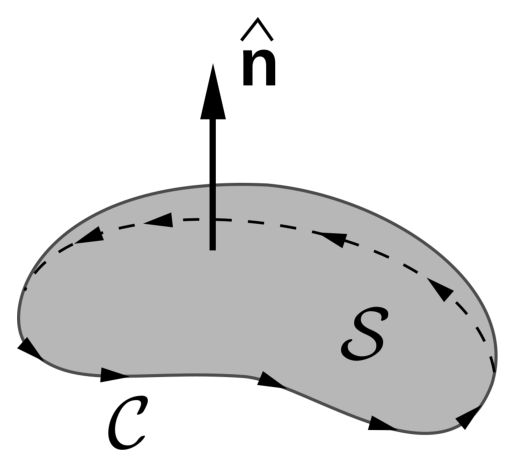
\includegraphics[width=1.5in]{modules/m0051_fStokesRHR.eps}
% https://en.wikipedia.org/wiki/File:Stokes'_Theorem.svg
}}{A curved surface with circumference labeled C, surface area labeled S, and normal vector pointing perpendicular to the surface. }
\end{center} 
\centerline{\scriptsize 
\copyright~\hyperref[m0051_fStokesRHR_Credit]{Cronholm144} (modified)
\href{https://creativecommons.org/licenses/by-sa/3.0/}{CC BY~SA 3.0} 
} 
\caption{
\label{m0051_fStokesRHR}
The relative orientations of the direction of integration ${\mathcal C}$ and surface normal $\hat{\bf n}$ in Stokes' Theorem.
}
\end{figure}

Stokes' Theorem is a purely mathematical result and not a principle of electromagnetics \emph{per se}.
The relevance of the theorem to electromagnetic theory is primarily as a tool in the associated mathematical analysis.
Usually the theorem is employed to transform a problem expressed in terms of an integration over a surface into an integration over a closed path or vice-versa.
For more information on the theorem and its derivation, see ``Additional Reading'' at the end of this section.

%%%%%%%%%%%%%%%%%%%%%%%%%%%%%%%%%%%%

{\bf Additional Reading:}
\begin{itemize}
\item ``\href{https://en.wikipedia.org/wiki/Stokes'_theorem}{Stokes' Theorem}'' on Wikipedia.
\end{itemize}

\index{Stokes' theorem|)}


